\documentclass[10pt,a4paper,spanish]{report}

\usepackage[spanish]{babel}
\usepackage[utf8]{inputenc}
\usepackage{amsmath, amsthm}
\usepackage{amsfonts, amssymb, latexsym}
\usepackage{enumerate}
\usepackage[official]{eurosym}
\usepackage{graphicx}
\usepackage[usenames, dvipsnames]{color}
\usepackage{colortbl}
\usepackage{multirow}
\usepackage{fancyhdr}
\usepackage[all]{xy}
\usepackage{pgfplots}
\usepackage{algpseudocode}
\usepackage{listings}
\usepackage{titlesec}

\pgfplotsset{compat=1.5}

% a4large.sty -- fill an A4 (210mm x 297mm) page
% Note: 1 inch = 25.4 mm = 72.27 pt
%       1 pt = 3.5 mm (approx)

% vertical page layout -- one inch margin top and bottom
\topmargin      0 mm    % top margin less 1 inch
\headheight     0 mm    % height of box containing the head
\headsep       10 mm    % space between the head and the body of the page
\textheight   250 mm
\footskip      14 mm    % distance from bottom of body to bottom of foot

% horizontal page layout -- one inch margin each side
%\oddsidemargin    0   mm    % inner margin less one inch on odd pages
%\evensidemargin   0   mm    % inner margin less one inch on even pages
%\textwidth      159.2 mm    % normal width of text on page

\usepackage[math]{iwona}
\usepackage[T1]{fontenc}
\usepackage{inconsolata}

\usepackage[pdftex, bookmarks=true,
	bookmarksnumbered=false, % true means bookmarks in
	% left window are numbered
	bookmarksopen=false,     % true means only level 1
	% are displayed.
	colorlinks=true,
linkcolor=webblue]{hyperref}

\definecolor{webgreen}{rgb}{0, 0.5, 0} % less intense green
\definecolor{webblue}{rgb}{0, 0, 0.5}  % less intense blue
\definecolor{webred}{rgb}{0.5, 0, 0}   % less intense red
\definecolor{dblackcolor}{rgb}{0.0,0.0,0.0}
\definecolor{dbluecolor}{rgb}{.01,.02,0.7}
\definecolor{dredcolor}{rgb}{0.8,0,0}
\definecolor{dgraycolor}{rgb}{0.30,0.3,0.30}

\newcommand{\HRule}{\rule{\linewidth}{0.5mm}} % regla horizontal para  el titulo

\pagestyle{fancy}
%con esto nos aseguramos de que las cabeceras de capítulo y de sección vayan en minúsculas

\renewcommand{\chaptermark}[1]{%
	\markboth{#1}{}}
\renewcommand{\sectionmark}[1]{%
	\markright{\thesection\ #1}}
\fancyhf{} %borra cabecera y pie actuales
\fancyhead[LREO]{\bfseries\thepage}
\fancyhead[LO]{\bfseries\leftmark}
\renewcommand{\headrulewidth}{0.5pt}
\renewcommand{\footrulewidth}{0pt}
\addtolength{\headheight}{0.5pt} %espacio para la raya
\fancypagestyle{plain}{%
	\fancyhead{} %elimina cabeceras en páginas "plain"
	\renewcommand{\headrulewidth}{0pt} %así como la raya
}

%%%%% Para cambiar el tipo de letra en el título de la sección %%%%%%%%%%%
\chapterfont{\fontfamily{pag}\selectfont} %% for chapter if you want
\sectionfont{\fontfamily{pag}\selectfont}
\subsectionfont{\fontfamily{pag}\selectfont}
\subsubsectionfont{\fontfamily{pag}\selectfont}
\titleformat{\chapter}{\normalfont\Huge}{}{0pt}{\Huge} % Capítulos sin "Capítulo x" encima del título

\renewcommand{\labelenumi}{\arabic{enumi}. }
\renewcommand{\labelenumii}{\labelenumi\alph{enumii}) }
\renewcommand{\labelenumiii}{\labelenumii\roman{enumiii}: }

\title{Seguridad y Protección de Sistemas Informáticos \\
Criptosistemas Simétricos}
\author{David Sánchez Jiménez}

\begin{document}
\begin{titlepage}
 \begin{center}
  \HRule \\[0.8cm]
  \textsc{\huge Seguridad y Protección \\ de Sistemas Informáticos \\[0.5cm] Criptosistemas Simétricos}\\[1.6cm]
  \HRule \\[1cm]
  \begin{flushleft}
   \emph{Hecho por:}\\
   David Sánchez Jiménez
  \end{flushleft}
  \vspace{12cm}
  \large{\today}\\
  \vspace{0.5cm}
  \htmladdnormallink{
\includegraphics[width=2cm]{Imagenes/88x31.png}}
  {http://creativecommons.org/licenses/by-nc/4.0/}\\[0.5cm]
  \texttt{Prácticas de Seguridad y Protección de Sistemas Informáticos\\ by
   \href{mailto:dasaji92@gmail.com}{David Sánchez Jiménez} is licensed under a \htmladdnormallink{Creative Commons Reconocimiento-NoComercial-CompartirIgual 4.0 Internacional License}
   {http://creativecommons.org/licenses/by-nc/4.0/}}.\\[3mm]
 \end{center}
\end{titlepage}

\tableofcontents
\newpage

% ----------------------------------------------------------------

\chapter{Ejercicio 1}

\section{Enunciado}
\noindent
Partiremos de un archivo binario de 1024 bits, todos ellos con valor 0. Para hacer referencia al mismo voy a suponer que se llama input.bin, pero podéis dar el nombre que os convenga.

\section{Respuesta}
\noindent
Para crear un archivo binario debemos abrir la terminal de Linux y escribir touch y el nombre del fichero que deseamos crear. \\

\begin{figure}[!hbp]
 \centering  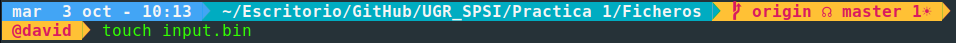
\includegraphics[width=1\textwidth]{./Imagenes/1.png}
\end{figure}

\noindent
A continuación abrimos dicho fichero con GHex y escribimos 128 parejas de 00, con esto ya tenemos los 1024 bits.

\begin{figure}[!hbp]
 \centering  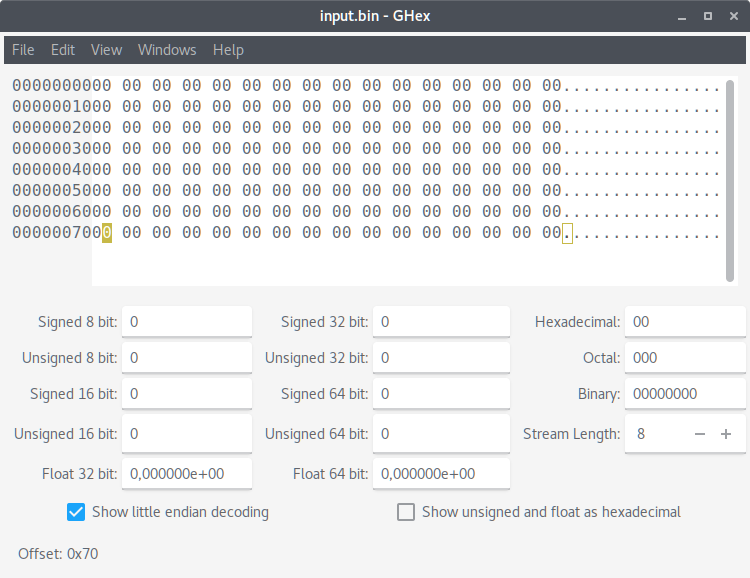
\includegraphics[width=1\textwidth]{./Imagenes/2.png}
\end{figure}

% ----------------------------------------------------------------

\chapter{Ejercicio 2}

\section{Enunciado}
\noindent
Creamos otro archivo binario del mismo tamaño, que contenga un único bit con valor 1 dentro de los primeros 40 bits y todos los demás con valor 0. Me referiré a este archivo como input1.bin

\section{Respuesta}

\noindent
De igual forma que en el ejercicio anterior creamos un nuevo archivo binario llamado input1.bin y le introducimos un bit con valor 1 dentro de los 40 primeros bits y los demás a 0.

\begin{figure}[!hbp]
 \centering  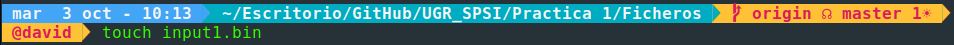
\includegraphics[width=1\textwidth]{./Imagenes/3.png}
\end{figure}

\begin{figure}[!hbp]
 \centering  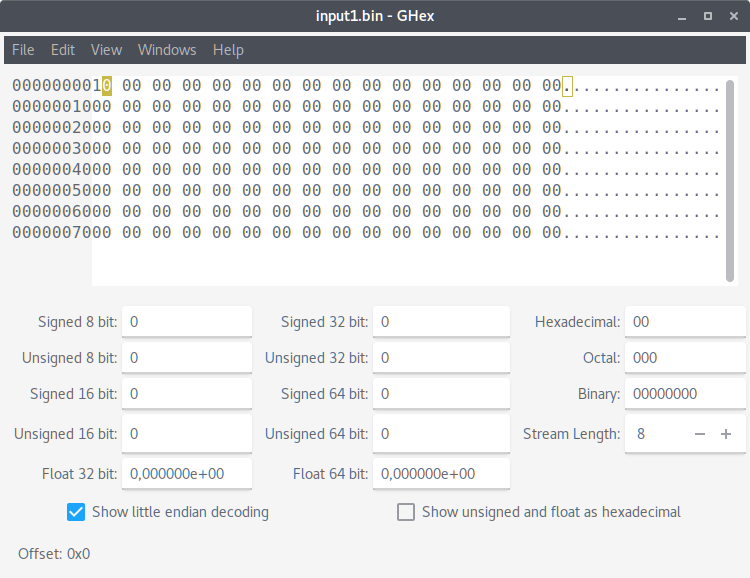
\includegraphics[width=1\textwidth]{./Imagenes/4.png}
\end{figure}

% ----------------------------------------------------------------

\chapter{Ejercicio 3}

\section{Enunciado}
\noindent
Cifrar input.bin con DES en modos ECB, CBC, OFB usando como claves una débil y otra semidébil, con vector de inicialización a vuestra elección y explicad los distintos resultados.

\section{Respuesta}
\noindent
Primero debemos cifrar el archivo input.bin con DES en modos ECB, CBC y OFB usando claves débiles y semidébiles como muestro a continuación. Las tres primeros corresponderían a los archivos cifrados usando una clave débil y los tres siguientes usando una clave semidébil.

\begin{figure}[!hbp]
 \centering  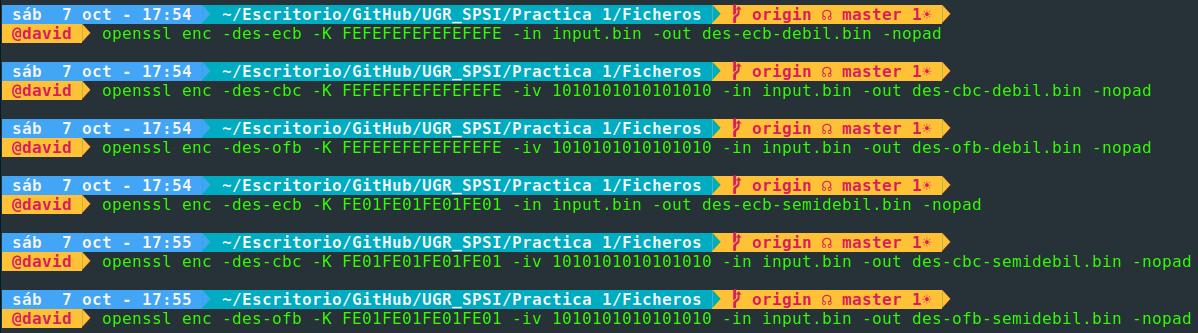
\includegraphics[width=1\textwidth]{./Imagenes/5.png}
\end{figure}

\newpage
\noindent
La primera salida corresponde al archivo cifrado con ECB utilizando una clave débil, en el cual el mensaje es dividido en bloques, cada uno de los cuales es cifrado de manera separada. Como todos los bloques sin cifrar son idénticos se producen idénticos textos cifrados. No utiliza vector de inicialización (IV). \\

\noindent
Las dos siguientes salidas corresponden con el archivo cifrado con CBC y OFB respectivamente utilizando una clave débil.\\

\noindent
En el modo CBC, antes de ser cifrado, a cada bloque de texto se le aplica una operación XOR con el previo bloque ya cifrado. Por lo que cada bloque cifrado depende de todos los bloques utilizados antes de el. Además, para hacer cada mensaje único se debe usar un vector de inicialización en el primer bloque.\\

\noindent
El modo OFB emplea una clave para crear un bloque pseudoaleatorio que es operado a través de XOR con el texto claro para generar el texto cifrado. Requiere de un vector de inicialización que debe ser único para cada ejecución realizada.

\begin{figure}[!hbp]
 \centering  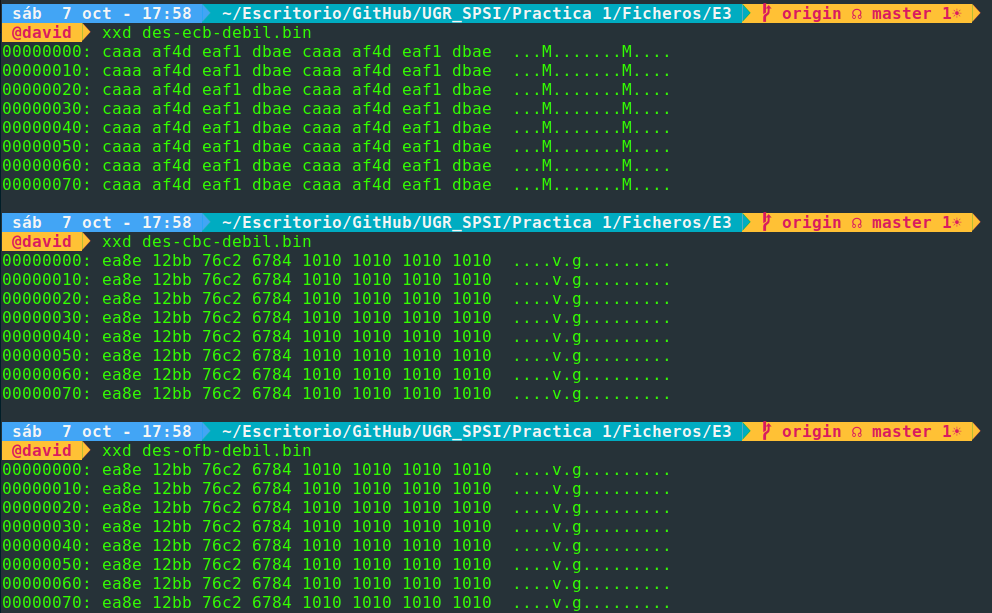
\includegraphics[width=1\textwidth]{./Imagenes/6.png}
\end{figure}

\noindent
Ahora pasamos a ver la codificación del archivo binario input.bin utilizando una clave semidébil, donde podemos observar el mismo comportamiento que en la imagen anterior.

\begin{figure}[!hbp]
 \centering  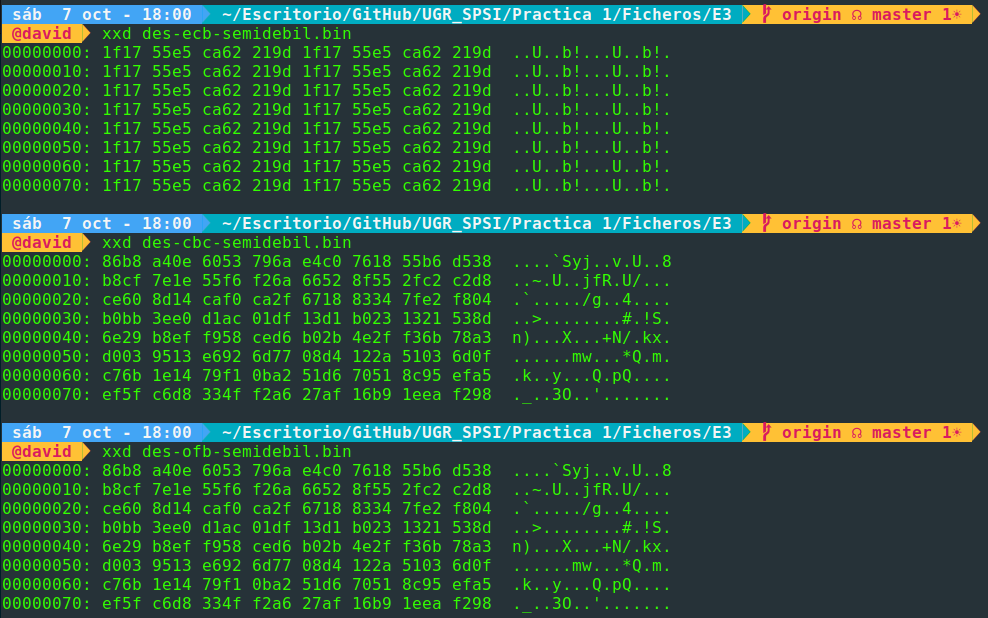
\includegraphics[width=1\textwidth]{./Imagenes/7.png}
\end{figure}

% ----------------------------------------------------------------


\chapter{Ejercicio 4}

\section{Enunciado}
\noindent
Cifrar input.bin e input1.bin con DES en modo ECB y clave a elegir, pero no débil ni semidébil. Explicad la forma de los resultados obtendos.

\section{Respuesta}
\noindent
Ciframos input.bin e input1.bin con DES en modo ECB utilizando una clave que no sea ni débil ni semidébil,en mi caso he utilizado 12AB89CD12AB89CD. \\

\noindent
Podemos observar que ambas salidas son iguales a excepción de los cuatro primeros bloques del primer vector del archivo cifrado correspondiente a input1.bin debido a que el archivo input.bin esta compuesto por solo valores 00 en input.bin mientras que el archivo input1.bin comienza por 10, por lo que el valor cifrado cambia.

\begin{figure}[!hbp]
 \centering  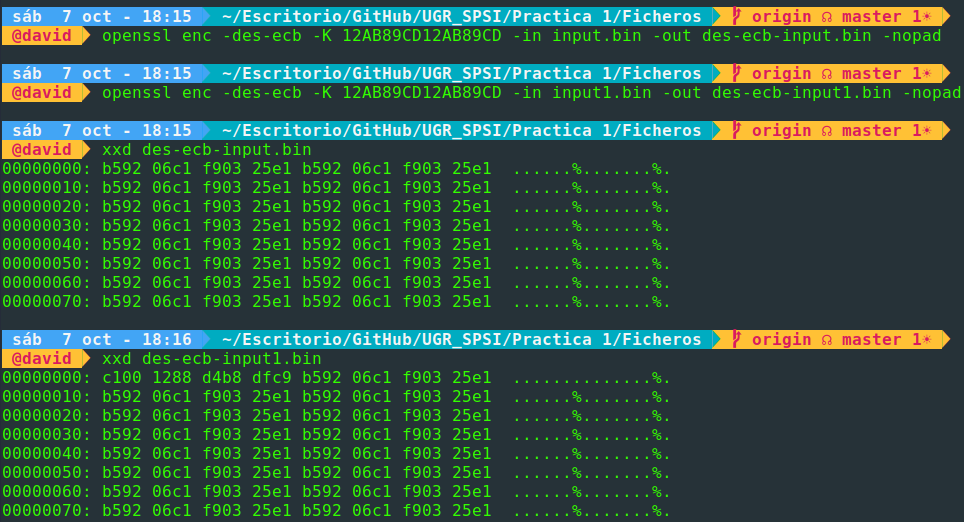
\includegraphics[width=1\textwidth]{./Imagenes/8.png}
\end{figure}

% ----------------------------------------------------------------

\chapter{Ejercicio 5}

\section{Enunciado}
\noindent
Cifrar input.bin e input1.bin con DES en modo CBC, clave y vector de inicialización a elegir. Comparad con los resultados obtenidos en el aparato anterior.

\section{Respuesta}
\noindent
Ciframos input.bin e input1.bin con DES en modo ECB utilizando una clave que no sea ni débil ni semidébil,en mi caso he utilizado 12AB89CD12AB89CD y el vector de inicialización 1010101010101010. \\

\noindent
En este caso podemos observar que las salidas de ambos archivos son diferentes debido a que al realizarse el cifrado se realiza una operación XOR al bloque previo ya cifrado, por lo que como el fichero input1.bin comienza por 10 y el fichero input.bin comienza por 00 pues las demás salidas son distintas.

\begin{figure}[!hbp]
 \centering  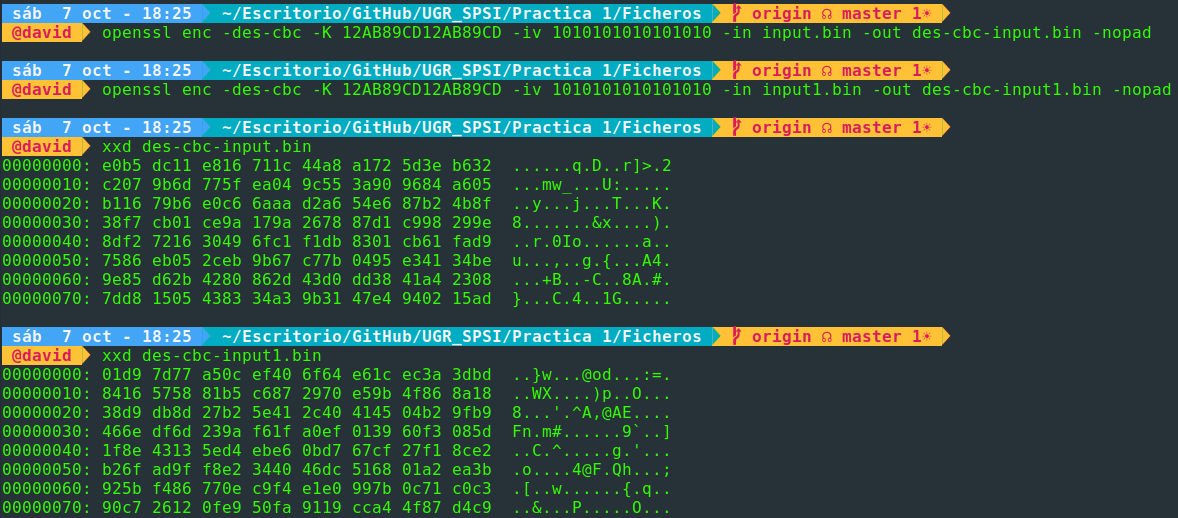
\includegraphics[width=1\textwidth]{./Imagenes/9.png}
\end{figure}

% ----------------------------------------------------------------

\chapter{Ejercicio 6}

\section{Enunciado}
\noindent
Repetid los puntos 4 a 5 con AES-128 y AES-256.

\section{Respuesta}
\noindent
En esta captura de pantalla se muestra el cifrado de input.bin y de input1.bin utilizando AES-128. \\

\noindent
En modo ECB podemos observar que los resultados de cifrar ambos archivos son iguales excepto el primer bloque de input1.bin que es diferente al resto.

\begin{figure}[!hbp]
 \centering  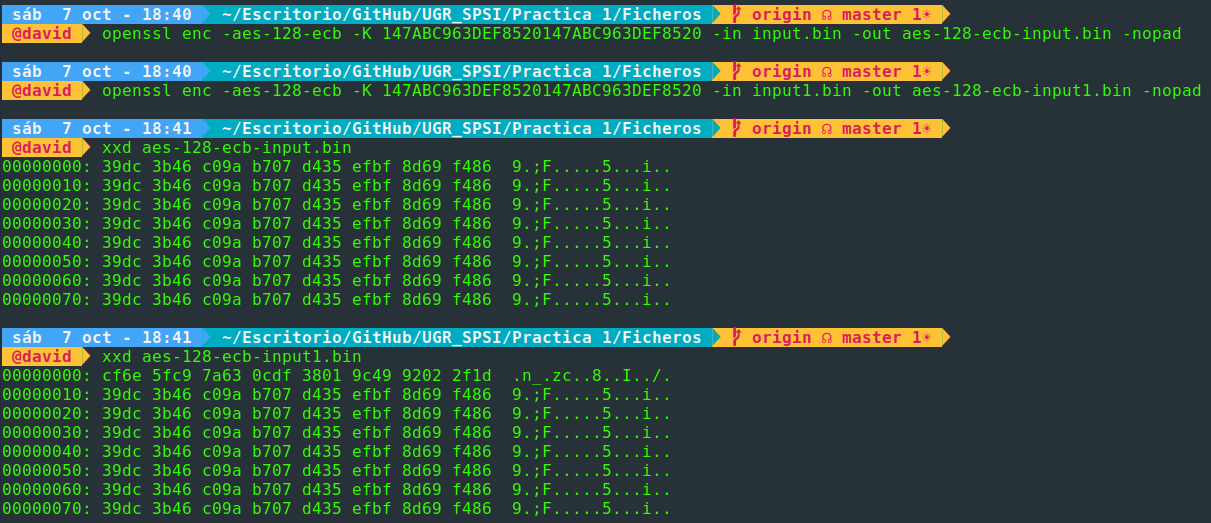
\includegraphics[width=1\textwidth]{./Imagenes/10.png}
\end{figure}

\noindent
En la salida del modo CBC podemos observar que ambos ficheros son totalmente distintos y que no siguen ningún patrón.

\begin{figure}[!hbp]
 \centering  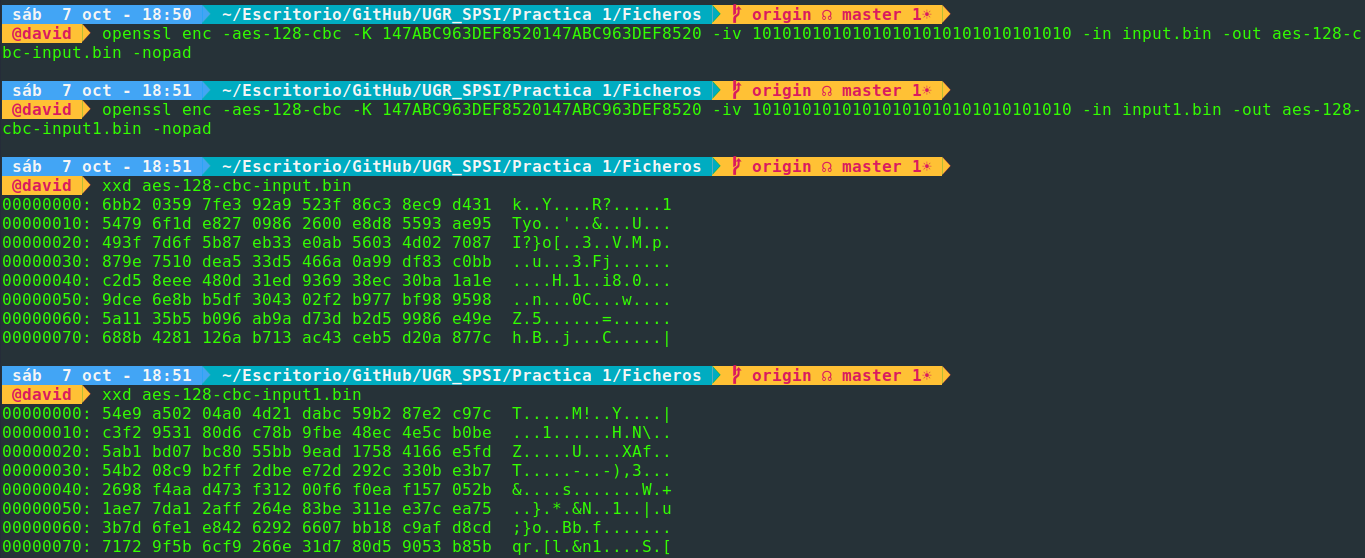
\includegraphics[width=1\textwidth]{./Imagenes/11.png}
\end{figure}

\newpage
\noindent
Ahora pasamos a cifrar ambos archivos utilizando AES-256.

\noindent
Observamos que al igual que en los casos anteriores al cifrar el archivo en modo ECB el resultado vuelve a ser el mismo a excepción del primer bloque de input1.bin.

\begin{figure}[!hbp]
 \centering  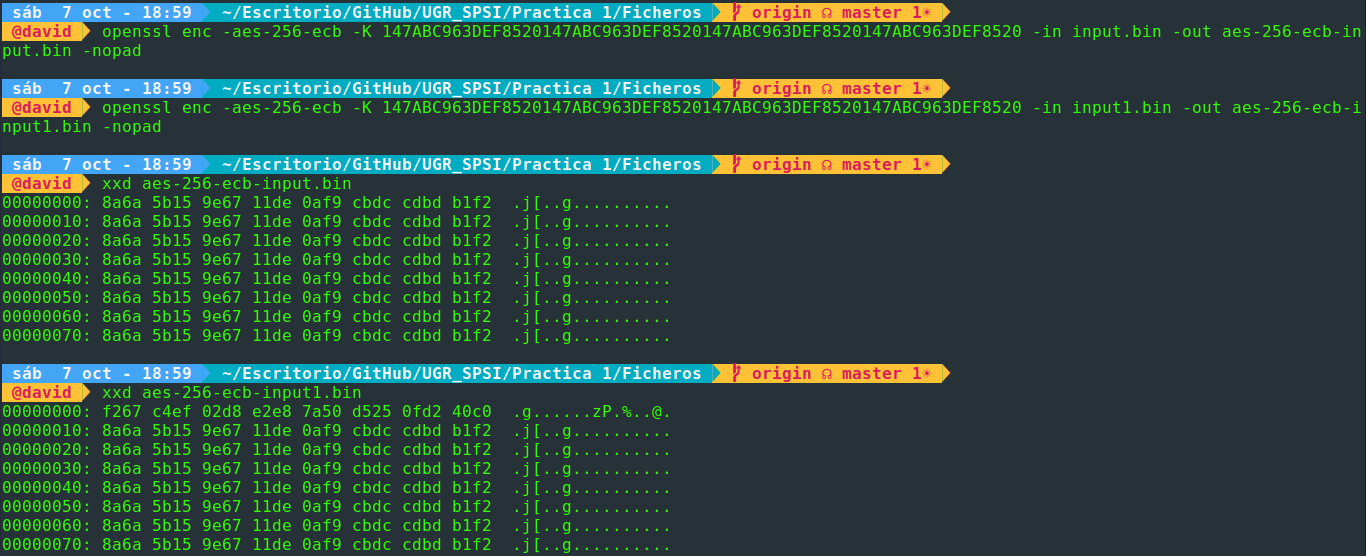
\includegraphics[width=1\textwidth]{./Imagenes/12.png}
\end{figure}

\noindent
El resultado obtenido al utilizar AES-256 es el mismo que en casos anteriores, ambas salidas son totalmente distintas y no siguen ningún patrón.

\begin{figure}[!hbp]
 \centering  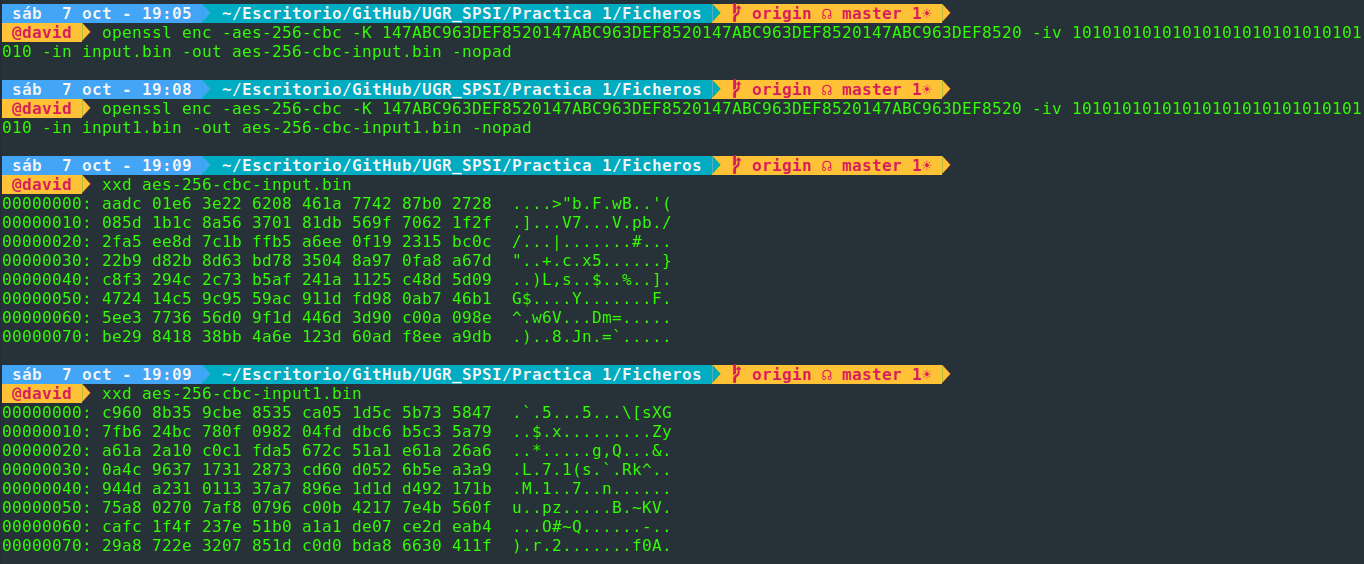
\includegraphics[width=1\textwidth]{./Imagenes/13.png}
\end{figure}

% ----------------------------------------------------------------

\chapter{Ejercicio 7}

\section{Enunciado}
\noindent
Cifrad input.bin con AES-192 en modo OFB, clave y vector de inicialización a elegir. Supongamos que la salida es output.bin.

\section{Respuesta}
\noindent
Ciframos el archivo input.bin con AES-192 en modo OFB como se muestra en la siguiente captura de pantalla.

\begin{figure}[!hbp]
 \centering  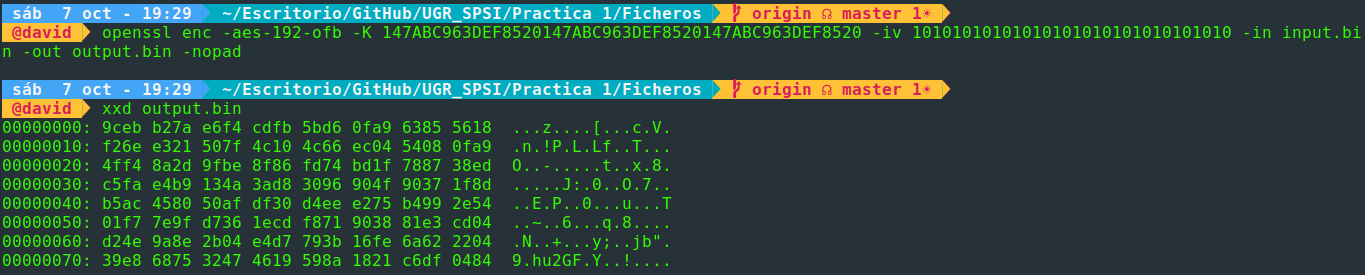
\includegraphics[width=1\textwidth]{./Imagenes/14.png}
\end{figure}

% ----------------------------------------------------------------

\chapter{Ejercicio 8}

\section{Enunciado}
\noindent
Descifra output.bin utilizando la misma clave y vector de inicialización que en el Ejercicio 7.

\section{Respuesta}
\noindent
Desciframos el archivo output.bin obtenido en el ejercicio anterior utilizando la opción -d y usando la misma clave y el vector de inicialización.

\begin{figure}[!hbp]
 \centering  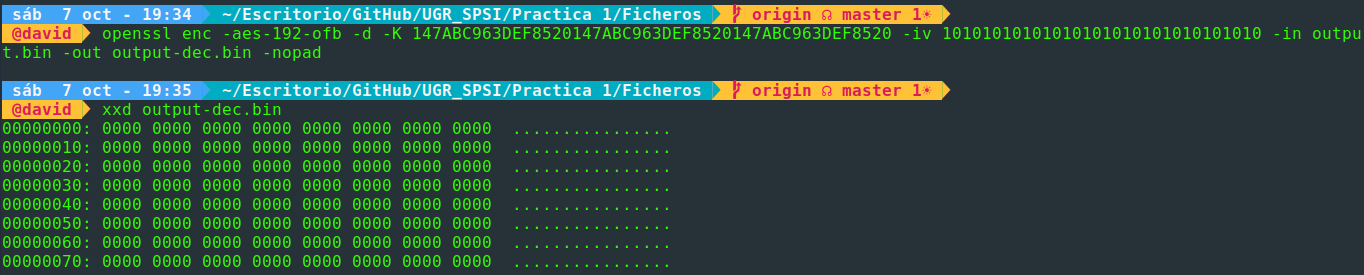
\includegraphics[width=1\textwidth]{./Imagenes/15.png}
\end{figure}

% ----------------------------------------------------------------

\chapter{Ejercicio 9}

\section{Enunciado}
\noindent
Vuelve a cifrar output.bin con AES-192 en modo OFB, clave y vector de inicialización del punto 7. Compara el resultado obtenido con el Ejercicio 8, explicando el resultado.

\section{Respuesta}
\noindent
Al volver a cifrar el archivo output.bin utilizando AES-192 en modo OFB y usando la misma clave y vector de inicialización obtenemos la misma salida que en el ejercicio anterior, ya que al ser simétrico el cifrado al volver a cifrar el mismo archivo bajo las mismas condiciones es equivalente a descifrarlo.

\begin{figure}[!hbp]
 \centering  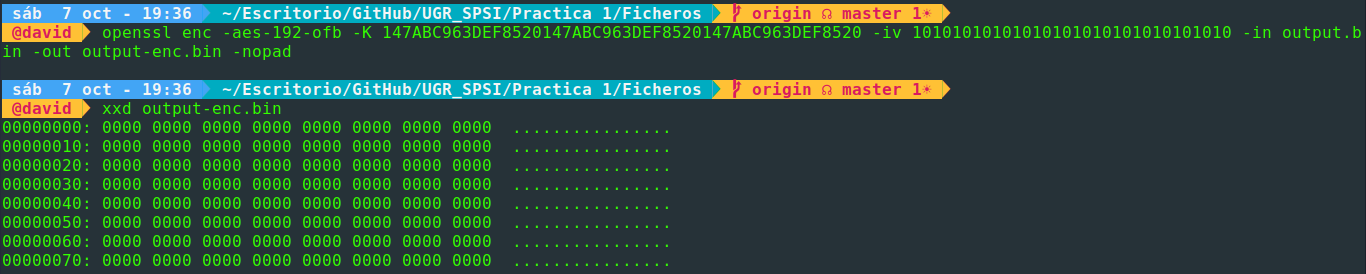
\includegraphics[width=1\textwidth]{./Imagenes/16.png}
\end{figure}

% ----------------------------------------------------------------

\chapter{Ejercicio 10}

\section{Enunciado}
\noindent
Presentad la descripción de otro cifrado simétrico que aparezca en vuestra implementación de OpenSSL.

\section{Respuesta}
\noindent
Voy a utilizar el cifrado BF (BlowFish) ya que acepta todos los modos de cifrado utilizados en los ejercicios anteriores. Este algoritmo esta compuesto por 18 semiclaves (K) y 4 cajas (subtitution boxes S). Es un proceso relativamente simple y altamente seguro ya que a la fecha no se conoce ningún tipo de criptoanalisis efectivo contra este algoritmo de cifrado.

% ----------------------------------------------------------------

\chapter{Ejercicio 11}

\section{Enunciado}
\noindent
Repetid los puntos 3 a 5 con el cifrado presentado en el punto 10 (el 3 si el cifrado elegido tuviese claves débiles o semidébiles).

\section{Respuesta}
\noindent
Ciframos el archivo input.bin con bf en modos ECB, CBC y OFB usando claves débiles y semidébiles como muestro a continuación.

\begin{figure}[!hbp]
 \centering  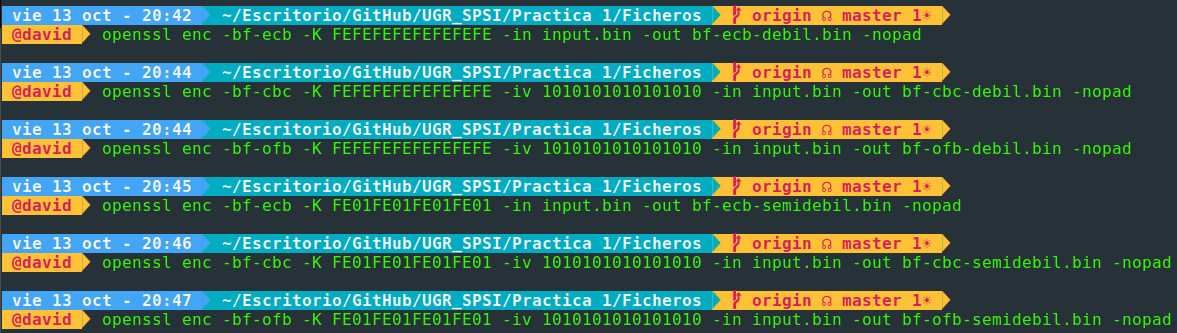
\includegraphics[width=1\textwidth]{./Imagenes/17.png}
\end{figure}

\noindent
Estas son las salidas ECB, CBC y OFB respectivamente obtenidos de cifrar archivo input.bin utilizando una clave débil.

\begin{figure}[!hbp]
 \centering  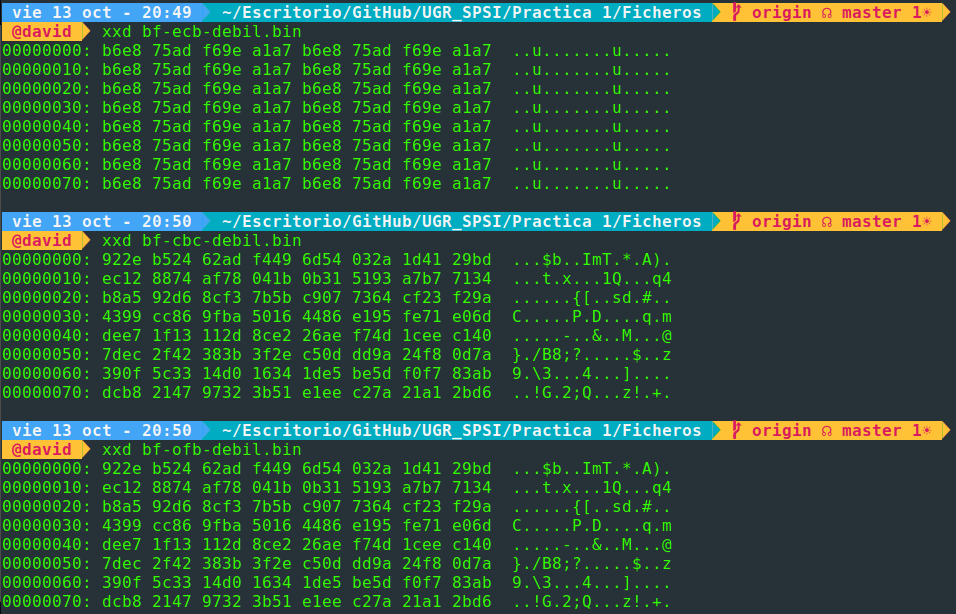
\includegraphics[width=1\textwidth]{./Imagenes/18.png}
\end{figure}

\newpage
\noindent
Estas son las salidas ECB, CBC y OFB respectivamente obtenidos de cifrar archivo input.bin utilizando una clave semidébil.

\begin{figure}[!hbp]
 \centering  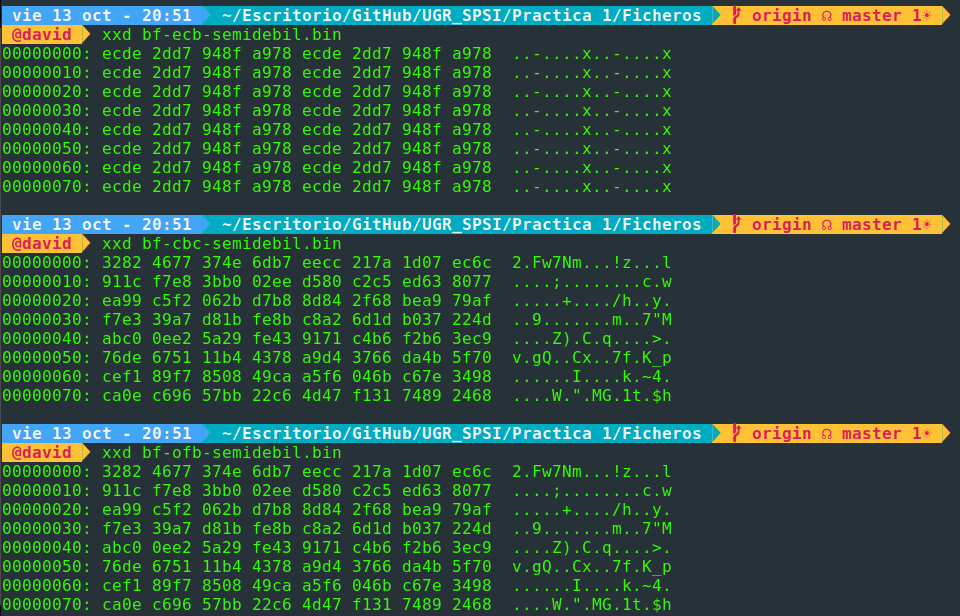
\includegraphics[width=1\textwidth]{./Imagenes/19.png}
\end{figure}

\noindent
Ahora pasamos a cifrar los archivos input.bin e input1.bin con bf en modo ECB y utilizando una clave que no es ni débil ni semidébil. \\

\noindent
Podemos observar que ambas salidas son iguales a excepción de los cuatro primeros bloques del primer vector del archivo cifrado correspondiente a input1.bin ya que este comienza por 10 y el archivo input.bin comienza por 00.

\begin{figure}[!hbp]
 \centering  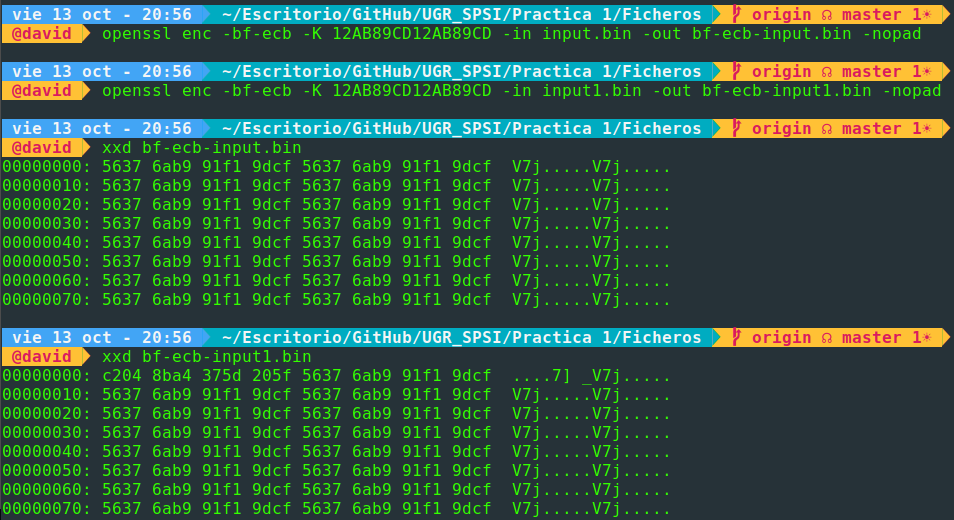
\includegraphics[width=1\textwidth]{./Imagenes/20.png}
\end{figure}

\newpage
\noindent
Ahora pasamos a cifrar los archivos input.bin e input1.bin con bf en modo CBC y utilizando una clave que no es ni débil ni semidébil. \\

\noindent
En este caso observamos que las salidas de ambos archivos son totalmente diferentes debido que al realizarse el cifrado se realiza una operación XOR al bloque previo ya cifrado, por lo que como el fichero input1.bin comienza por 10 y el fichero input.bin comienza por 00 pues las demás salidas son distintas.

\begin{figure}[!hbp]
 \centering  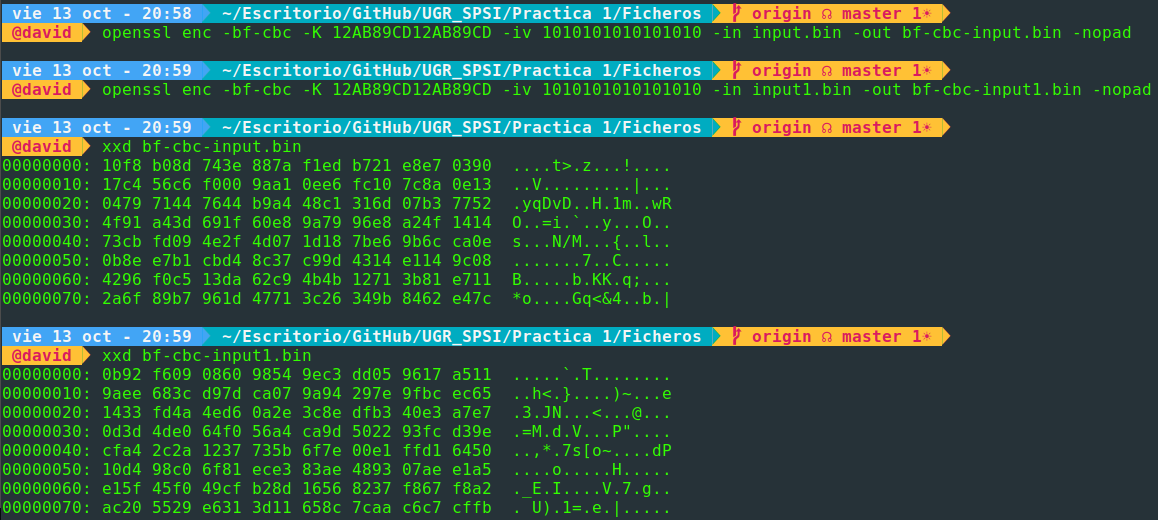
\includegraphics[width=1\textwidth]{./Imagenes/21.png}
\end{figure}


% ----------------------------------------------------------------
\end{document}
